\setlength{\columnsep}{3pt}
\begin{flushleft}
\begin{itemize}
	\item lscpu: Command to display CPU details.
	\begin{tcolorbox}[breakable,notitle,boxrule=-0pt,colback=pink,colframe=pink]
		\color{black}
		\fontdimen2\font=9pt
		Syntax: lscpu
		\fontdimen2\font=4pt
	\end{tcolorbox}
	Eg:
	\begin{figure}[h!]
		\centering
		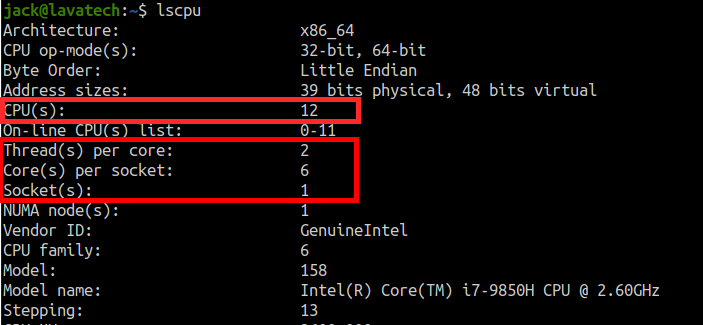
\includegraphics[scale=.45]{content/chapter12/images/cpu1.png}
		\caption{Sample output}
		\label{fig:cpu1}
	\end{figure}
	
	Output explaination: Here,
	\begin{itemize}
		\item Number of physical CPU(s) = 6
		\item Number of logical CPU(s) = 12
	\end{itemize}	
	
	\begin{figure}[h!]
		\centering
		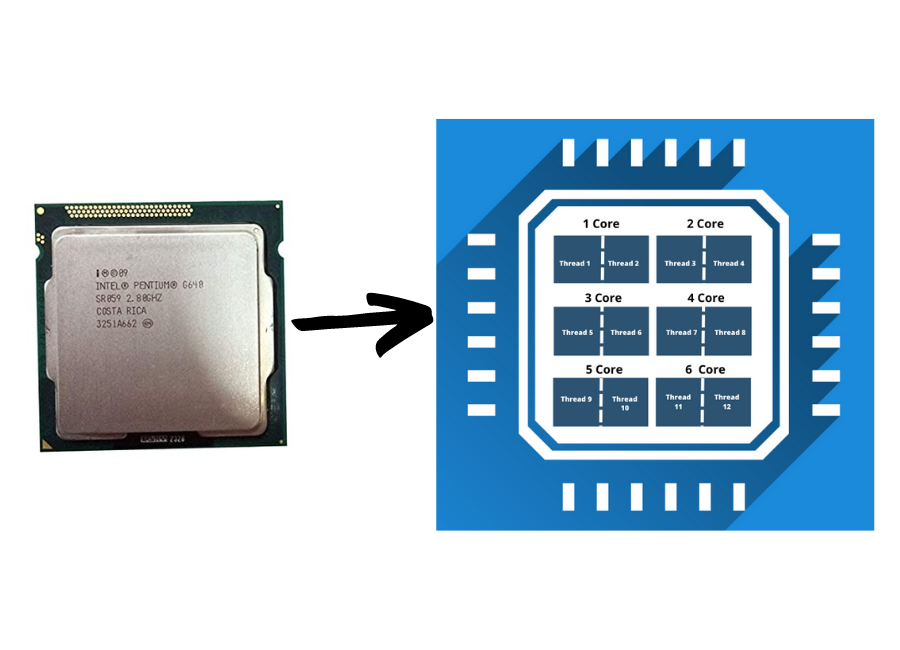
\includegraphics[scale=.45]{content/chapter12/images/intel.png}
		\caption{Sample output}
		\label{fig:cpu1}
	\end{figure}
	\newpage
	
	\item \textbf{iostat}: Reports CPU statistics and I/O statistics for devices and partitions.
	\newline
	Options with \textbf{iostat} command:
	\begin{itemize}
		\item \textbf{-c}: Displays CPU utilization report.
		\bigskip
		\begin{tcolorbox}[breakable,notitle,boxrule=0pt,colback=pink,colframe=pink]
			\color{black}
			\fontdimen2\font=9pt
			Syntax: iostat -c
			\fontdimen2\font=4pt
		\end{tcolorbox}
		Eg:
		\begin{figure}[h!]
			\centering
			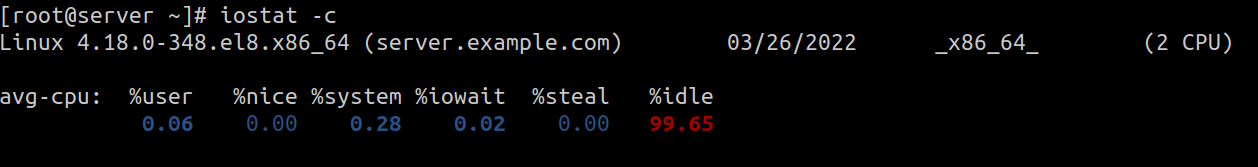
\includegraphics[scale=0.2]{content/chapter15/images/iostat.png}
			\caption{Sample output}
			\label{fig:output}
		\end{figure}
		
		Output explaination:
		\begin{itemize}
			\item \textbf{\%user}: Show CPU utilization of user application.
			\item \textbf{\%nice}: Show CPU utilization of user application with nice priority.
			\item \textbf{\%system}: Show CPU utilization of the system kernel.
			\item \textbf{\%iowait}: Show CPUs idle percentage during outstanding disk I/O request.
			\item \textbf{\%steal}: Show wait by the virtual CPUs while the hypervisor was servicing another virtual processor.
			\item \textbf{\%ideal}: Show CPUs idle percentange when the	system did not have an outstanding disk I/O request.
		\end{itemize}
	\end{itemize}
	\newpage
	\item \textbf{vmstat}: 
	\begin{itemize}
		\item Stands for \textbf{V}irtual \textbf{M}emory \textbf{STAT}stics.
		\item It is a computer monitoring tool that collects and displays system memory, processes, interrupts, pagging and block I/O.
	\end{itemize}
	\bigskip
	Option with \textbf{vmstat} command:
	\newline
	\textbf{-s}: Displays a table of event counters and memory statistics.
	\newline
	\begin{tcolorbox}[breakable,notitle,boxrule=0pt,colback=pink,colframe=pink]
		\color{black}
		\fontdimen2\font=9pt
		Syntax: vmstat -s
		\fontdimen2\font=4pt
	\end{tcolorbox}
	Eg:
	\begin{figure}[h!]
		\centering
		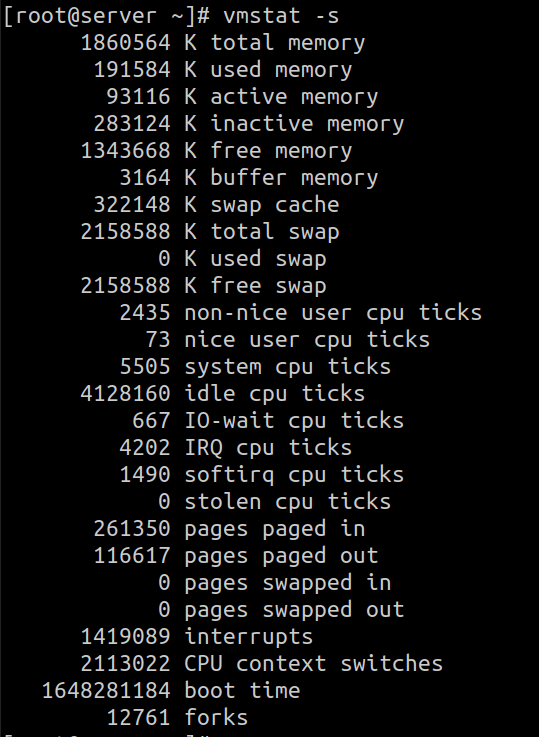
\includegraphics[scale=0.4]{content/chapter15/images/vmstat.png}
		\caption{Sample output}
		\label{fig:output3}
	\end{figure}
	
	\newpage
	\item \textbf{sar}: 
	\begin{itemize}
		\item The \textbf{sar} command is a performance monitoring uitility.
		\item It collects reports ongoing basis and saves the performance data.
		\begin{tcolorbox}[breakable,notitle,boxrule=0pt,colback=pink,colframe=pink]
			\color{black}
			\fontdimen2\font=9pt
			Syntax: sar
			\fontdimen2\font=4pt
		\end{tcolorbox}
		Eg:
		\begin{figure}[h!]
			\centering
			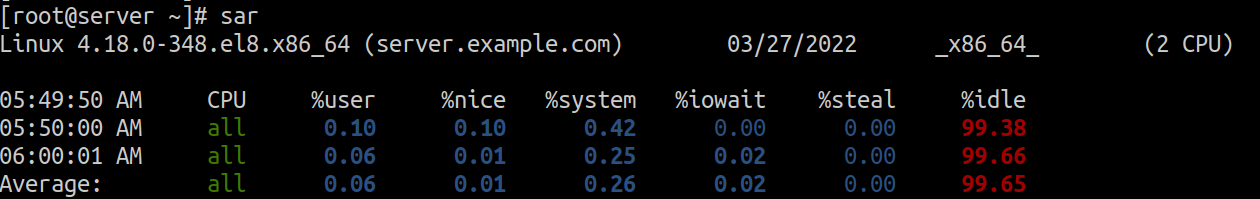
\includegraphics[scale=0.25]{content/chapter15/images/sar.png}
			\caption{Sample output}
			\label{fig:output4}
		\end{figure}
		
		Refer \textbf{iostat} command for output explaination.	
		


\end{itemize}
\end{flushleft}

\newpage


